\documentclass[10pt]{article}

\usepackage[utf8]{inputenc}
\usepackage[T1]{fontenc}
\usepackage[margin=1in]{geometry}
\usepackage{hyperref}
\usepackage{url}
\usepackage{booktabs}
\usepackage{amsmath}
\usepackage{amsfonts}
\usepackage{nicefrac}
\usepackage{microtype}
\usepackage{graphicx}
\usepackage{multirow}
\usepackage{float}
\usepackage{natbib}
\usepackage{titlesec}
\usepackage{parskip}

\titleformat{\section}{\large\bfseries}{\thesection}{1em}{}
\titleformat{\subsection}{\normalsize\bfseries}{\thesubsection}{1em}{}
\setlength{\parskip}{4pt}

\title{\textbf{Optimizing Urban Traffic Efficiency with Reinforcement Learning}}

\author{
  Jialin Cai \quad Zhiyan Chen \quad Yunzhao Li \quad An Zhou \\[4pt]
  Department of Statistical and Actuarial Sciences, Western University \\
  London, Canada \\
  \texttt{\{jcai256, zche264, yli4333, azhou257\}@uwo.ca}
}
\date{April 15, 2026}

\begin{document}
\maketitle

% ── Abstract ──────────────────────────────────────────────────────────────────
\begin{abstract}
Fixed-time traffic signal controllers waste green time on empty approaches
while vehicles queue on the other side — a problem that grows worse as demand
becomes more variable.  We formulate adaptive signal control as a Markov
Decision Process and train two deep reinforcement learning agents — a Double
Dueling DQN and a Proximal Policy Optimization (PPO) agent — to minimise
vehicle waiting time and maximise throughput at a single 4-way intersection.
The core intuition is simple: a controller only needs to learn \emph{which
direction has more waiting vehicles} to substantially outperform a fixed plan,
and this mapping is easy for a small neural network to acquire from experience.
We validate on two simulators: SUMO (moderate load, high fidelity) and CityFlow
(near-saturation, fast).  On SUMO, DQN reduces average queue length by
\textbf{46.3\%} and increases throughput by \textbf{11.4\%} over the fixed
baseline.  On CityFlow, PPO achieves a \textbf{9.6\%} reward improvement.
Code is available at \url{https://github.com/ashzyc/CS9170-RL-Traffic-Efficiency}.
\end{abstract}

% ── 1. Introduction ───────────────────────────────────────────────────────────
\section{Introduction}

Traffic congestion in urban areas imposes enormous economic and environmental
costs.  Over 300,000 signalised intersections exist in the United States
alone~\citep{schrank2021tti}, and the majority still use \emph{fixed-time}
controllers: phase sequences and durations are computed offline from historical
flow data and hardcoded into the controller.  Such plans are optimal only under
the conditions assumed at design time; stochastic, non-stationary real-world
demand routinely violates those assumptions.

\paragraph{Why existing techniques fall short.}
Actuated controllers extend a phase while loop detectors sense approaching
vehicles, but react to single-point measurements and cannot reason about
downstream queue build-up.  Analytical methods such as Webster's
formula~\citep{webster1958} minimise average delay under steady-state Poisson
arrivals — an assumption that rarely holds in practice.  Model predictive
control requires an accurate dynamic traffic model that must be re-calibrated
continuously as demand patterns shift.

\paragraph{Intuition behind our approach.}
The fundamental insight is that the optimal switching decision reduces to a
single question: \emph{which direction currently has more frustrated vehicles?}
A controller that always serves the heavier queue will outperform a fixed plan
without needing an explicit traffic model.  The challenge is that queue states
evolve stochastically and the reward for a good decision arrives several steps
after the action.  Deep RL handles this naturally: an agent learns the
queue-to-action mapping from experience, and an experience replay buffer
lets it revisit past transitions to build a stable value function despite
the delayed feedback.

\paragraph{Contributions.}
\begin{itemize}
  \item We implement Double Dueling DQN and PPO, comparing both against a
        fixed-time baseline on a 4-way intersection.
  \item We evaluate on SUMO (moderate load) and CityFlow (near-saturation)
        to understand how traffic utilisation affects the benefit of adaptive control.
  \item We provide a fully reproducible codebase with one-line scripts for
        training, evaluation, and live GUI demonstration.
\end{itemize}

% ── 2. Related Work ───────────────────────────────────────────────────────────
\section{Related Work}

\paragraph{DQN for traffic signal control.}
\citet{li2016traffic} were among the first to apply deep Q-networks to adaptive
signal control, demonstrating that a queue-length policy can match hand-tuned
Webster timings.  \citet{wei2018intellilight} introduced IntelliLight, a
practical DQN agent with interpretable reward shaping that outperforms fixed
plans on travel time and queue length.

\paragraph{Pressure-based reward.}
\citet{wei2019presslight} replaced queue-length rewards with a \emph{pressure}
signal — the difference in vehicle densities across the stop line — showing
faster convergence under saturation.  This motivates our reward term penalising
total vehicles in the network (Equation~\ref{eq:reward}).

\paragraph{Multi-intersection coordination.}
\citet{wei2019colight} and \citet{chen2020toward} scale DQN to city-wide
networks via graph attention and decentralised learners.  Our single-intersection
work is a prerequisite for such extensions.

\paragraph{Policy gradient methods.}
\citet{liang2019deep} demonstrated that PPO converges reliably for multi-phase
signal control.  The clipped surrogate of \citet{schulman2017proximal} and
GAE of \citet{schulman2015high} underpin our PPO implementation.

\paragraph{Simulation platforms.}
\citet{zhang2019cityflow} introduced CityFlow for RL research;
\citet{behrisch2011sumo} describe SUMO's microscopic simulation with GUI replay.
We use both to test whether learned policies transfer across simulator fidelity.

% ── 3. Methods ────────────────────────────────────────────────────────────────
\section{Methods}

\subsection{Problem Formulation}

We model the intersection as an MDP
$(\mathcal{S}, \mathcal{A}, \mathcal{P}, \mathcal{R}, \gamma)$.

\textbf{State} $s_t \in \mathbb{R}^{11}$:
\begin{equation}
s_t = [\,v_N,\, v_S,\, v_E,\, v_W,\;
        w_N,\, w_S,\, w_E,\, w_W,\;
        V_{\text{total}},\; W_{\text{total}},\; \phi_t\,]
\end{equation}
where $v_d$ is the vehicle count on approach $d$, $w_d$ the halting count,
$V_{\text{total}}$ and $W_{\text{total}}$ are network totals, and
$\phi_t \in \{0,1\}$ is the active phase.  All normalised to $[0,1]$.

\textbf{Action} $a_t \in \{0, 1\}$: NS green (0) or EW green (1).
A 3-step yellow transition is enforced on every phase switch.

\textbf{Reward}:
\begin{equation}
r_t = (W_{t-1} - W_t) - 0.05\,V_t, \quad r_t \in [-10,\,10]
\label{eq:reward}
\end{equation}
Rewards reductions in halting vehicles and penalises vehicles still in the
network.  Discount $\gamma = 0.95$; episode length 200 steps.

\subsection{Double Dueling DQN}

Our DQN combines three improvements over vanilla DQN~\citep{mnih2015human}.

\textbf{Double DQN}~\citep{van2016deep} decouples action selection from
evaluation using a frozen target network:
\begin{equation}
y_t = r_t + \gamma\,Q_{\theta^-}\!\bigl(s_{t+1},\;
      \arg\max_a Q_\theta(s_{t+1}, a)\bigr)
\end{equation}

\textbf{Dueling architecture}~\citep{wang2016dueling} decomposes $Q$ into
state-value and advantage streams:
\begin{equation}
Q(s,a;\theta) = V(s;\theta_v) +
A(s,a;\theta_a) - \tfrac{1}{|\mathcal{A}|}\textstyle\sum_{a'}A(s,a';\theta_a)
\end{equation}

\textbf{Experience replay} (capacity 10,000, minibatch 64) with Huber loss.
The replay buffer is key: it lets DQN reuse each transition many times across
training, building a stable value function even when rewards are sparse.

\subsection{Proximal Policy Optimization}

Shared actor-critic backbone (128-128, orthogonal init).  Actor outputs a
categorical distribution over $\{0,1\}$; critic estimates state value.

GAE~\citep{schulman2015high}: $\hat{A}_t = \sum_{l \ge 0}(\gamma\lambda)^l
\delta_{t+l}$, $\;\delta_t = r_t + \gamma V(s_{t+1}) - V(s_t)$, $\lambda{=}0.95$.

\begin{equation}
\mathcal{L}^{\text{CLIP}} =
\mathbb{E}_t\!\left[\min\!\left(
  \rho_t\hat{A}_t,\;
  \text{clip}(\rho_t,\,1{-}\epsilon,\,1{+}\epsilon)\hat{A}_t
\right)\right], \quad \epsilon=0.2
\end{equation}

Unlike DQN, PPO is on-policy: each rollout is discarded after 4 gradient
epochs, so every transition is seen at most 4 times before being discarded.

\subsection{Hyperparameters}

\begin{table}[H]
\centering
\caption{Hyperparameter settings.}
\label{tab:hyper}
\begin{tabular}{lcc}
\toprule
\textbf{Parameter} & \textbf{DQN} & \textbf{PPO} \\
\midrule
Hidden layers              & 128-128           & 128-128 \\
Optimiser / lr             & Adam / $10^{-3}$  & Adam / $3{\times}10^{-4}$ \\
Discount $\gamma$          & 0.95              & 0.95 \\
$\varepsilon$ (start$\to$min) & $1.0\to0.05$ & — \\
$\varepsilon$ decay        & 0.99/ep           & — \\
Replay buffer / batch      & 10,000 / 64       & — \\
Target net update          & every 10 ep       & — \\
PPO clip $\epsilon$        & —                 & 0.2 \\
GAE $\lambda$              & —                 & 0.95 \\
Entropy coeff.             & —                 & 0.01 \\
Rollout / PPO epochs       & —                 & 200 / 4 \\
Training episodes          & 300               & 300 \\
\bottomrule
\end{tabular}
\end{table}

\subsection{Fixed-Time Baseline}

Alternates phases every 30 steps regardless of queue state, approximating
standard pre-timed plans.

\subsection{Simulation Environments}

\textbf{SUMO}: 4-way intersection (2 lanes, 50\,km/h), demand 300\,veh/h
straight and 100\,veh/h turning per direction.  Moderate utilisation; rewards
range $-300$ to $-400$/episode.  Controlled via Python TraCI.

\textbf{CityFlow}: benchmark single-intersection with heavier demand operating
near saturation; rewards range $-1700$ to $-2000$/episode.  The large
difference in reward scale between simulators reflects congestion level, not a
difference in the reward formula — both use Equation~\ref{eq:reward}.
CityFlow runs ${\sim}10{\times}$ faster than SUMO.

% ── 4. Evaluation ─────────────────────────────────────────────────────────────
\section{Evaluation}

\subsection{Training Dynamics}

\begin{table}[H]
\centering
\caption{Mean episode reward (first vs.\ last 50 training episodes).}
\label{tab:training}
\begin{tabular}{lcccc}
\toprule
 & \multicolumn{2}{c}{\textbf{SUMO}} & \multicolumn{2}{c}{\textbf{CityFlow}} \\
\cmidrule(lr){2-3}\cmidrule(lr){4-5}
\textbf{Method} & First 50 & Last 50 & First 50 & Last 50 \\
\midrule
Fixed-time & $-352.9$ & $-352.9$ & $-1982.4$ & $-1982.4$ \\
DQN        & $-347.3$ & $\mathbf{-313.3}$ & $-1978.4$ & $-1983.3$ \\
PPO        & $-387.7$ & $-393.3$ & $-1828.0$ & $\mathbf{-1774.5}$ \\
\bottomrule
\end{tabular}
\end{table}

On SUMO, DQN improves from $-347$ to $-313$ and converges by episode 260.
PPO starts lower and drifts to $-393$, below the fixed baseline.  The
divergence traces to update strategy: DQN's replay buffer recycles each
transition many times, efficiently building a stable value function.  PPO
discards each rollout after 4 epochs, forcing constant re-exploration of a
delayed-reward environment.

On CityFlow the roles reverse.  DQN's Q-values converge to near-identical
estimates for both actions (the near-flat saturation landscape gives no
learning signal), effectively degenerating to a fixed policy.  PPO's relative
advantage estimates retain a weak but exploitable directional gradient,
yielding a gradual improvement ($-1828 \to -1775$).

\begin{figure}[H]
  \centering
  \begin{minipage}[b]{0.48\textwidth}
    \centering
    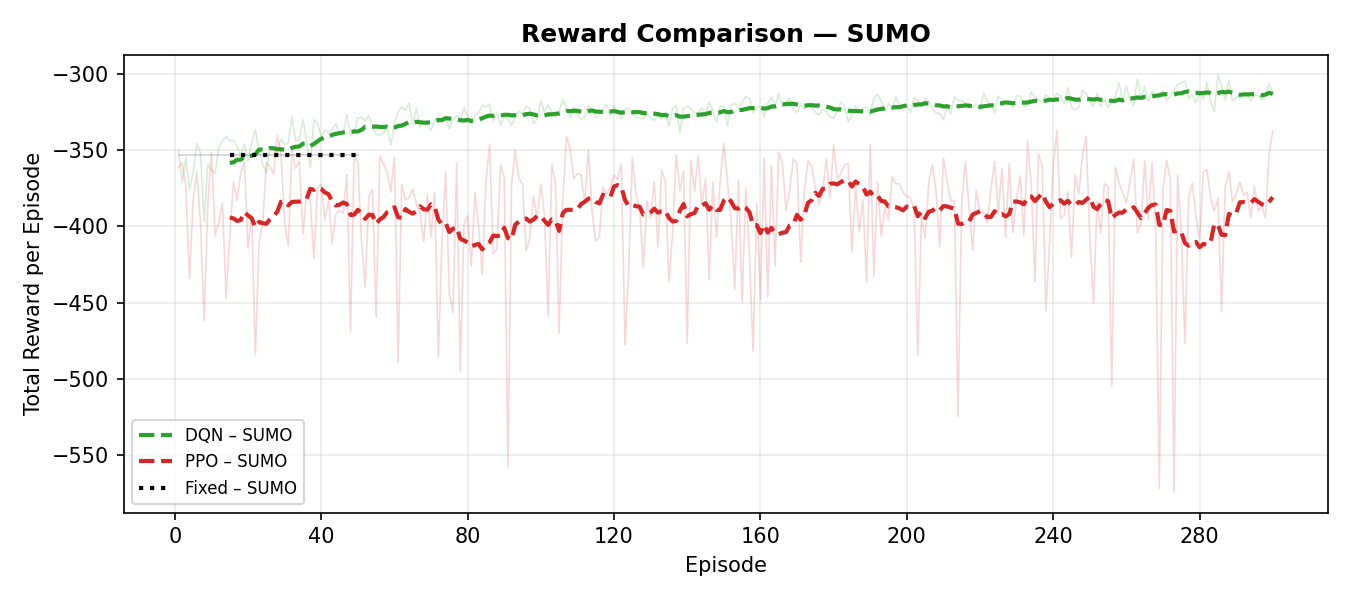
\includegraphics[width=\textwidth]{../results/comparison_sumo.png}
    \caption{SUMO training curves. DQN converges above fixed-time; PPO degrades.}
    \label{fig:train_sumo}
  \end{minipage}
  \hfill
  \begin{minipage}[b]{0.48\textwidth}
    \centering
    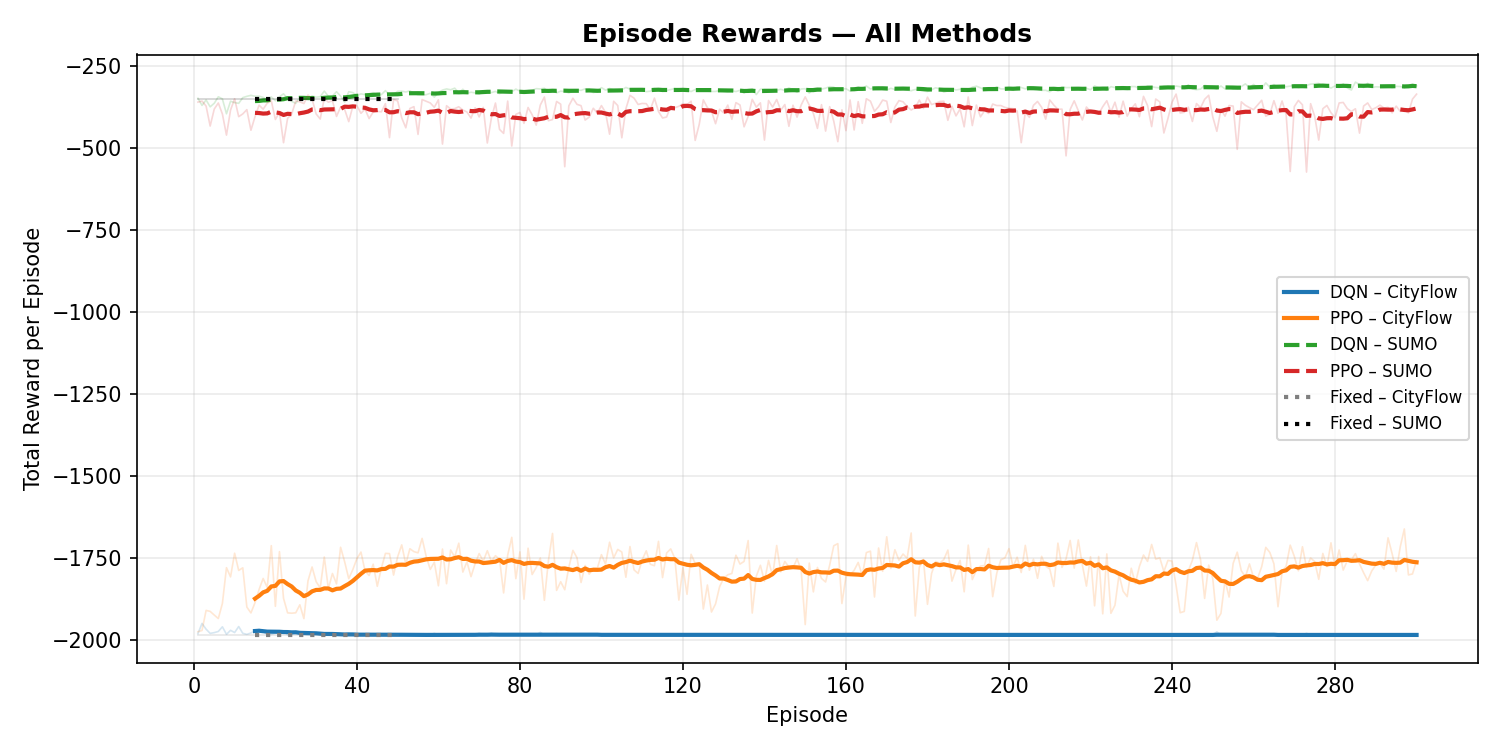
\includegraphics[width=\textwidth]{../results/comparison_rewards.png}
    \caption{CityFlow training curves. PPO improves gradually; DQN is flat.}
    \label{fig:train_cityflow}
  \end{minipage}
\end{figure}

\subsection{Final Performance}

\begin{table}[H]
\centering
\caption{Evaluation over 10 held-out episodes (best checkpoint).}
\label{tab:eval}
\begin{tabular}{lrrrrr}
\toprule
 & \multicolumn{3}{c}{\textbf{SUMO (moderate load)}} &
   \multicolumn{2}{c}{\textbf{CityFlow (near-saturation)}} \\
\cmidrule(lr){2-4}\cmidrule(lr){5-6}
\textbf{Method} & Reward & Queue & Throughput & Reward & Queue \\
\midrule
Fixed-time & $-352.9$ & $6.03$ & $1{,}018$ & $-1982.4$ & $449.6$ \\
DQN  & $\mathbf{-312.5}$ & $\mathbf{3.24}$ & $\mathbf{1{,}134}$ & $-1983.6$ & $446.6$ \\
PPO  & $-374.2$ & $7.60$ & $1{,}112$ & $\mathbf{-1791.9}$ & $469.6$ \\
\bottomrule
\end{tabular}
\end{table}

\begin{figure}[H]
  \centering
  \begin{minipage}[b]{0.48\textwidth}
    \centering
    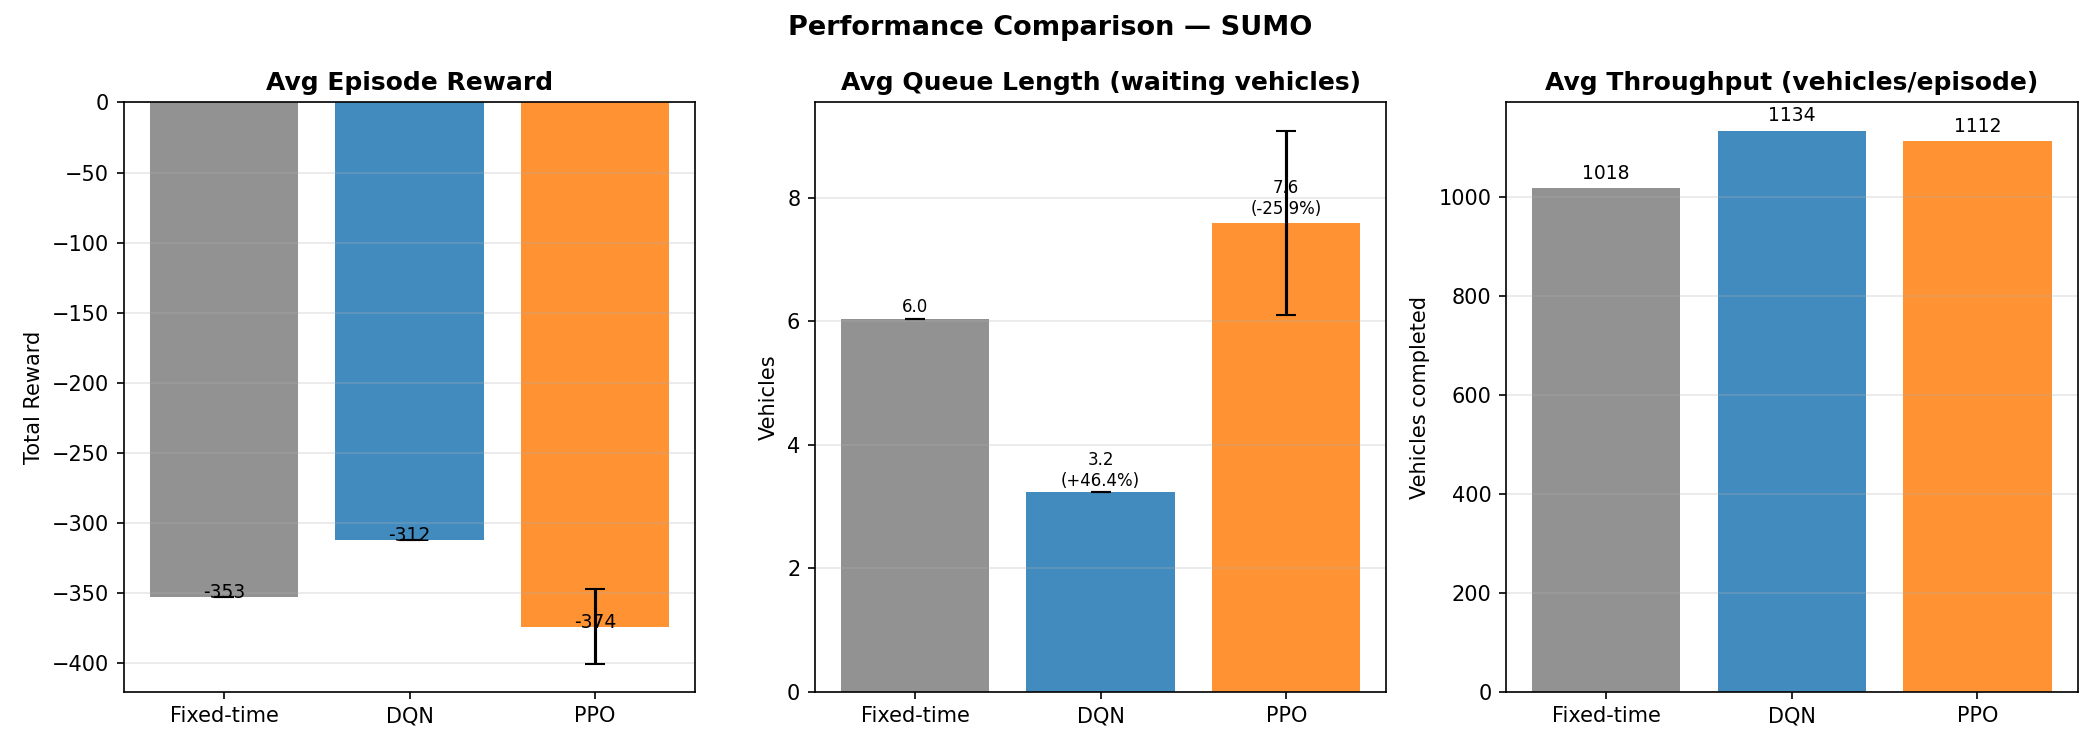
\includegraphics[width=\textwidth]{../results/evaluation_sumo.png}
    \caption{SUMO evaluation. DQN leads on all three metrics.}
    \label{fig:eval_sumo}
  \end{minipage}
  \hfill
  \begin{minipage}[b]{0.48\textwidth}
    \centering
    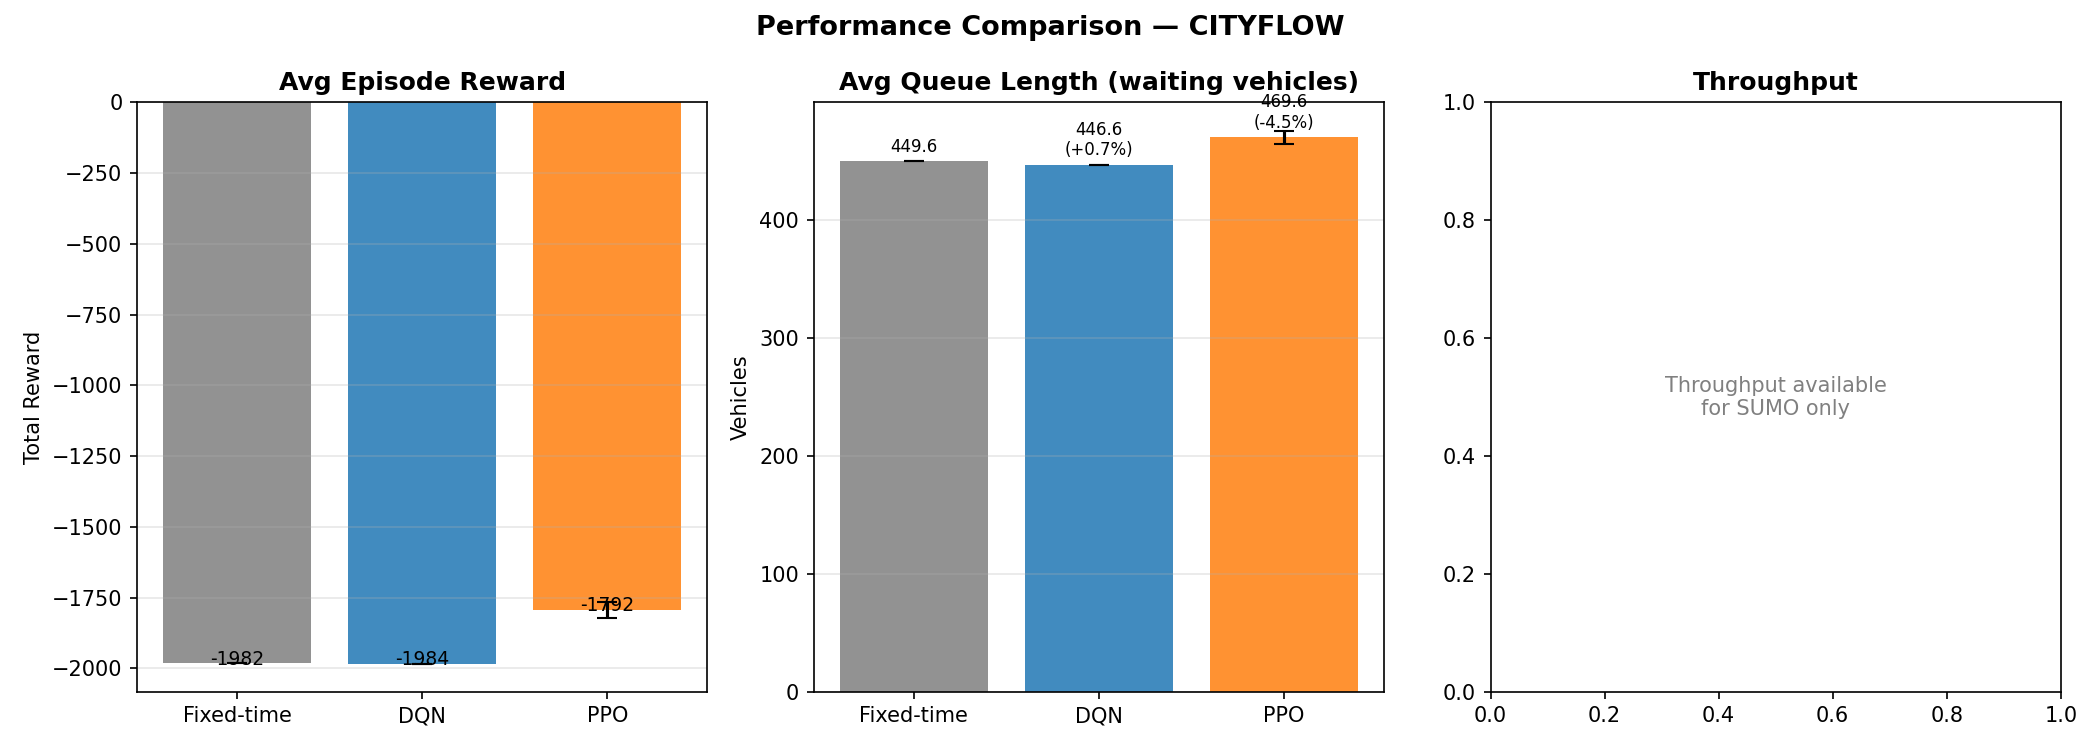
\includegraphics[width=\textwidth]{../results/evaluation_cityflow.png}
    \caption{CityFlow evaluation. PPO achieves best reward; DQN matches fixed.}
    \label{fig:eval_cityflow}
  \end{minipage}
\end{figure}

\paragraph{SUMO.}
DQN achieves \textbf{11.4\%} reward improvement, \textbf{46.3\%} queue
reduction ($3.24$ vs.\ $6.03$), and \textbf{11.4\%} throughput increase.
The replay buffer is the deciding factor: DQN learns that holding the
heavier-queue direction until it clears outperforms mechanical alternation.
PPO ends below the fixed baseline — without a replay buffer it never
stabilises a consistent policy on this delayed-reward task.

\paragraph{CityFlow.}
Under near-saturation, both approaches are permanently congested so the fixed
plan performs nearly as well as any binary policy can.  DQN's Q-values
degenerate; PPO's relative advantage signal survives, yielding a
\textbf{9.6\%} reward gain with high variance.

\subsection{Signal Phase Analysis}

\begin{figure}[H]
  \centering
  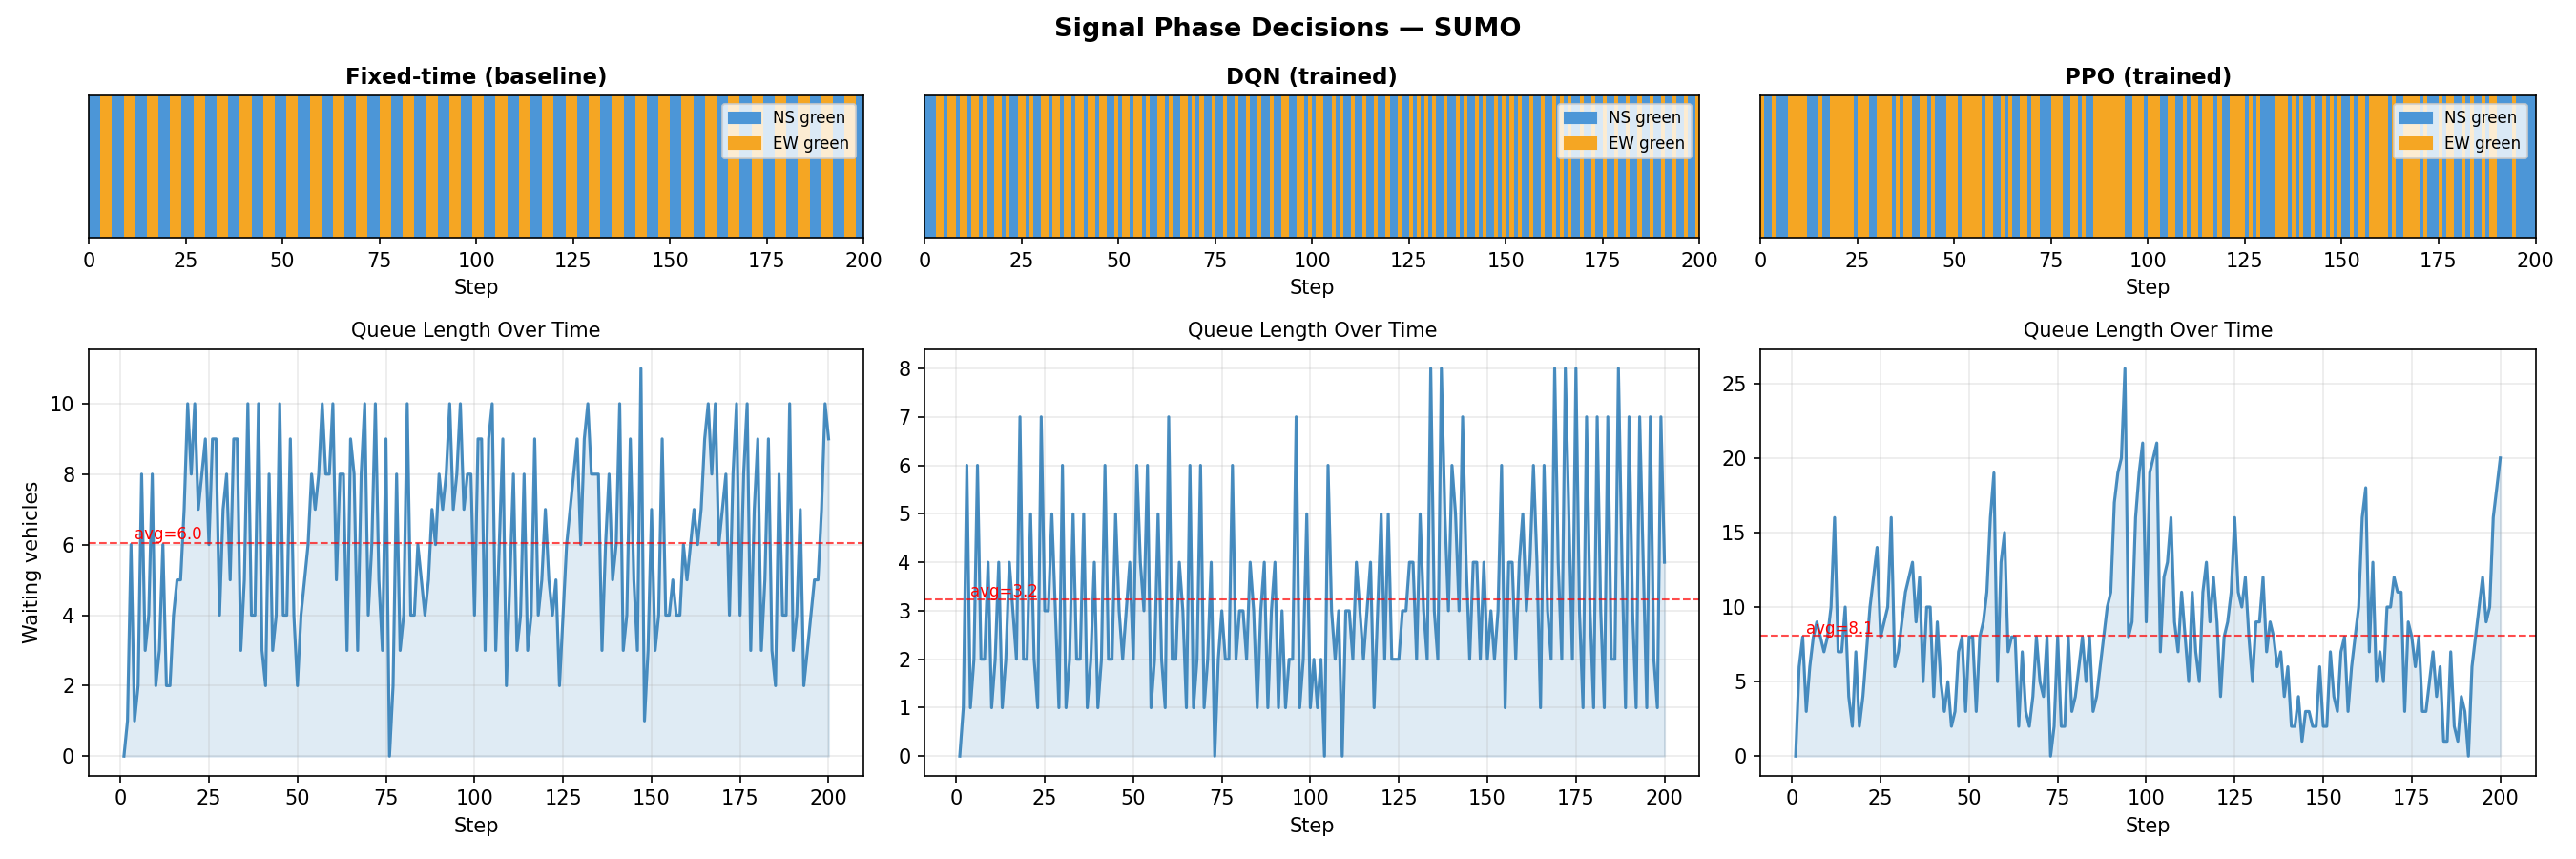
\includegraphics[width=0.72\textwidth]{../results/phase_timeline_sumo.png}
  \caption{Phase decisions and queue traces over 200 steps (SUMO).
  \textbf{Top}: fixed-time (rigid 30-step alternation).
  \textbf{Middle}: DQN (holds dominant phase until queue clears).
  \textbf{Bottom}: PPO (excessive switching, yellow-transition overhead).}
  \label{fig:phases}
\end{figure}

Figure~\ref{fig:phases} shows phase decisions on SUMO.  DQN qualitatively
replicates the max-pressure policy~\citep{wei2019presslight}: it extends the
green on the heavier-demand direction until the backlog clears.  PPO switches
far more frequently, often within a single action period; the resulting
yellow-phase overhead reduces effective green time and explains its poor SUMO
performance.

% ── 5. Conclusion ─────────────────────────────────────────────────────────────
\section{Conclusion}

\paragraph{Can RL effectively tackle adaptive signal control?}
Yes, under moderate load.  DQN cuts queue length by 46\% and boosts throughput
by 11\% on SUMO by learning one key behaviour: serve the heavier queue and
hold the phase until it clears.  Under near-saturation (CityFlow), this
advantage shrinks because both directions are always congested; PPO ekes out a
9.6\% reward improvement where DQN cannot.  The practical takeaway: adaptive RL
control delivers the greatest benefit precisely in the regimes where fixed plans
are most obviously broken — moderate and highly variable load — and a
sample-efficient off-policy algorithm (DQN) is preferable when rewards are
sparse and delayed.

\paragraph{Limitations.}
Single intersection, symmetric stationary demand, binary action space.

\paragraph{Future work.}
\begin{itemize}
  \item Multi-intersection MARL with graph attention~\citep{wei2019colight}.
  \item Variable phase durations (not just which phase, but for how long).
  \item Pressure-based reward~\citep{wei2019presslight} for better saturation performance.
  \item Real-world demand calibrated from loop-detector logs.
\end{itemize}

\paragraph{Acknowledgements.}
Code: \url{https://github.com/ashzyc/CS9170-RL-Traffic-Efficiency}.
No external funding received.

\bibliographystyle{plainnat}
\bibliography{../references}

\end{document}
